\documentclass[12pt]{article}

% --- Packages ---
\usepackage[utf8]{inputenc}
\usepackage[T1]{fontenc}
\usepackage[english]{babel}
\usepackage{graphicx}
\usepackage{geometry}
\usepackage{hyperref}
\usepackage{enumitem}
\usepackage{titlesec}
\usepackage{setspace}
\geometry{a4paper, margin=1in}
\onehalfspacing 

% --- Project Details ---
\title{
    \vspace{-1in}
    \begin{center}
        \textbf{CE 216: Fundamental Topics in Programming I} \\
        \vspace{0.1in}
        \large{Spring 2026}
    \end{center}
    \vspace{0.4in}
    Milestone 1: Design and Architecture Document \\
    \textbf{Sports Manager Project}
}

\author{
    \textbf{Instructor: Assoc. Prof. Dr. Kaya Oğuz} \\
    \vspace{0.3in}
    \textbf{Group: Final Four} \\ \\
    \begin{tabular}{ll}
        \textbf{Name Surname} & \textbf{Student ID} \\
        \hline
        Bilgenur Memiş & 20240602050 \\
        Elif Güneş Tüzer & 20240602072 \\
        Selim Baltacı & 20230602011 \\
        Rabia Tülay Gökdağ  & 20210602029 \\
    \end{tabular}
}
\date{March 15, 2026}


\begin{document}

\maketitle
\newpage
\tableofcontents
\newpage

% --- SECTION 1: INTRODUCTION ---
\section{Introduction}
Sports management games allow players to take the role of a team manager instead of directly controlling athletes during matches. In these games, the player makes decisions such as choosing the team lineup, managing players, and setting strategies that may affect the outcome of the matches. Because of this, the main challenge is not playing the sport itself but managing the team successfully throughout the season.

The goal of this project is to develop a Sports Manager application with a graphical user interface (GUI). The application will simulate a league environment where teams, players, and matches are organized within the system. Additionally, the application will use AI-generated data such as player and coach names, team names, and logos to make the game environment more realistic and visually engaging.

To support maximum flexibility, the project separates the user interface from the sport-specific logic. The interface interacts with the game through abstract structures and Java interfaces instead of depending on a specific sport implementation. This design allows new sports to be added without changing the user interface.

% --- SECTION 2: SYSTEM ARCHITECTURE ---
\section{System Architecture}

\subsection{Core Goals}
The framework is built to support multiple sports (like Volleyball or Headball) without the need to rewrite the entire system every time a new one is added.
\begin{itemize}
    \item \textbf{Open for Extension:} New sports can be added easily without changing the core engine’s code.
    \item \textbf{Separation of Concerns:} Sport rules, visuals (UI), and game logic are kept separate to prevent bugs and messy code.
    \item \textbf{High Extensibility:} Using standard Java tools (interfaces and abstract classes), new sports can be "plugged in" seamlessly to the existing structure.
\end{itemize}

\subsection{Layered Architecture}
The system follows a rigid four-layer structure to ensure modularity and facilitate independent development of game components.

\subsubsection{UI Layer}
The UI Layer is entirely decoupled from the business logic, interacting exclusively with the \texttt{ISport} interface to maintain sport-agnosticism. This layer supports specific data-binding requirements, including the rendering of team logos and the management of AI-generated assets, such as names for players and coaches loaded from external sources.

\subsubsection{Game Logic Layer}
This layer governs the simulation lifecycle and competition organization through three primary components: the \texttt{MatchEngine} for outcome calculation, the \texttt{League} for automated fixture generation, and the \texttt{Match} class for tracking individual event execution and scores.

\subsubsection{Sport Layer}
The Sport Layer serves as the rule-set abstraction, centered on the \texttt{ISport} interface. This interface acts as a mandatory contract, forcing concrete implementations like \texttt{FootballSport} and \texttt{HeadballSport} to define critical parameters via specific methods.

\subsubsection{Data Layer}
This layer defines the persistence hierarchy and entity state. The \texttt{BasePlayer} abstract class serves as the entity foundation, encapsulating shared attributes including age, fitness, and injury status. Conversely, the \texttt{BaseTeam} class acts as a container for these entities.

\newpage

% --- SECTION 3: CORE CLASSES ---
\section{Core Classes}
This section describes the core classes of the Sports Manager application. The design relies heavily on abstraction and object-oriented principles to ensure flexibility and modularity.

\subsection{Interfaces and Sport Rules}
\subsubsection{ISport (Interface)}
The \texttt{ISport} interface defines the general structure and rules that every sport must follow. It follows the \textbf{Open-Closed Principle}, allowing new sports to be introduced without modifying the engine.
\begin{itemize}
    \item \texttt{getRequiredPlayers()}: Returns the number of players required for a team.
    \item \texttt{getMatchDuration()}: Returns the duration of a match.
    \item \texttt{getPointForWin()}: Returns the points awarded for a win.
\end{itemize}

\subsubsection{FootballSport}
A concrete implementation of \texttt{ISport} defining football-specific rules, such as 11-player teams and standard durations. It remains independent of the UI and game management components.

\subsubsection{HeadballSport}
Another implementation of \texttt{ISport} representing a fictional sport. It demonstrates the system's flexibility as the game engine treats it identically to football via the interface contract.

\subsection{Entity Hierarchy}
\subsubsection{BasePlayer (Abstract Class)}
An abstract foundation for generic players. It cannot be instantiated directly and contains shared attributes:
\begin{itemize}
    \item \texttt{name, age, fitness, isInjured}
    \item \textbf{Methods:} \texttt{train()} to improve fitness and \texttt{recover()} to handle fatigue/injury.
\end{itemize}

\subsubsection{FootballPlayer and HeadballPlayer}
These classes extend \texttt{BasePlayer}. While inheriting common attributes, they allow for sport-specific properties like tactical roles or skill ratings.

\subsubsection{BaseTeam}
Acts as a container for multiple player entities. It manages the \texttt{teamName}, the roster list, and total league \texttt{points}.

\subsection{Simulation and Management}
\subsubsection{Match}
Represents a game between two teams. It tracks \texttt{homeScore}, \texttt{awayScore}, and the \texttt{isPlayed} status. The \texttt{playMatch()} method triggers the simulation process.

\subsubsection{MatchEngine}
The core simulation component. It determines outcomes based on team strength, fitness, and sport rules using the \texttt{simulateMatch(team1, team2, rules)} method.

\subsubsection{League}
The central manager of the competition. It maintains the list of teams, generates the schedule via \texttt{generateFixture()}, and updates rankings through \texttt{updateStandings()}.

\newpage

% --- SECTION 4: UML CLASS DIAGRAM ---
\section{UML Class Diagram}
The following diagram shows the system architecture and class interactions.

\begin{figure}[h]
    \centering
    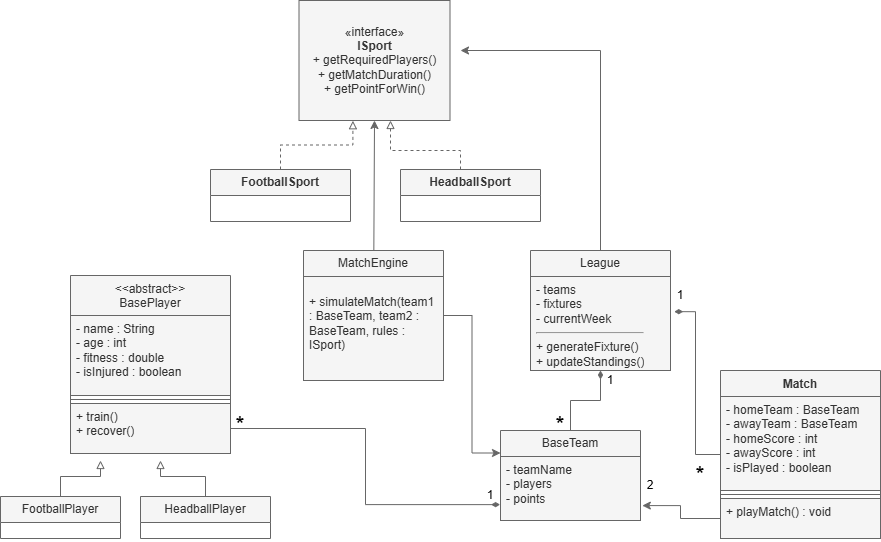
\includegraphics[width=0.85\textwidth]{uml_diagram.png} 
    \caption{UML Class Diagram of the Sports Manager Framework}
    \label{fig:uml}
\end{figure}

\subsection{UML Coordination and Technical Directives}
\begin{itemize}
    \item \textbf{Interfaces:} The \texttt{ISport} interface is designated with the \textit{<<interface>>} stereotype.
    \item \textbf{Abstract Classes:} The \texttt{BasePlayer} class is identified as abstract via italics.
    \item \textbf{Inheritance:} Solid arrows with empty triangular heads show inheritance from \texttt{BasePlayer}.
    \item \textbf{Composition/Aggregation:} The \texttt{League} aggregates \texttt{BaseTeam} instances and maintains composition with \texttt{Match} entities.
\end{itemize}

\newpage

% --- SECTION 5: USER INTERFACE DESIGN ---
\section{User Interface Design}
The UI is designed for clarity and usability. It is completely separate from the core game logic and interacts only through the \texttt{ISport} interface and system classes.

\subsection{Key Screens}
\begin{itemize}
    \item \textbf{Main Menu:} Launch screen to start games or select sports.
    \item \textbf{Team Screen:} Displays team info, logos, and squad data from \texttt{BaseTeam}.
    \item \textbf{League Table:} Shows updated standings managed by the \texttt{League} class.
    \item \textbf{Match Screen:} Displays scores calculated by the \texttt{MatchEngine}.
    \item \textbf{Player List:} Lists player attributes from classes extending \texttt{BasePlayer}.
\end{itemize}

% --- SECTION 6: EXTENSIBILITY ---
\section{Extensibility}
Since the game logic only communicates through the \texttt{ISport} interface, adding a new sport like Volleyball is as simple as writing a new class that implements the interface. Nothing else in the system needs to change.

% --- SECTION 7: CONCLUSION ---
\section{Conclusion}
This project builds a flexible simulation by layering the UI, logic, and rules. The result is a clean, maintainable foundation that follows OOP principles and can grow as the project develops.

\end{document}
